\section{Appendix 2: Energy subtraction due to upstream material}\label{appendix:EnergyCorrections}
%%%%%%%%%%%%%%%%%%%%%%%%%%%%%%%%%%%%%%%%%%%%%%%%%%%%%%%%%%%%%%%%

Figure \ref{fig:EndPointPionMCInBeamLine} shows the end point position for the single particle $\pi$ Monte Carlo launched from $z=-100$~cm. This ``x-ray'' plot demonstrates the upstream material that is present in the LArIAT simulation of the beamline. While a large number of the simulated particles manage to enter the TPC, they will interact with the material and thus lose energy prior to being measured in the TPC.

\begin{figure}[h!]
\centering
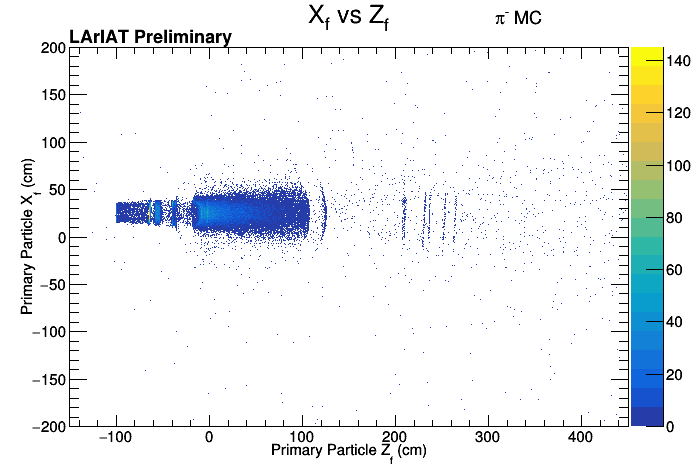
\includegraphics[scale=0.45]{./images/UnweightedXfvsZf.png}
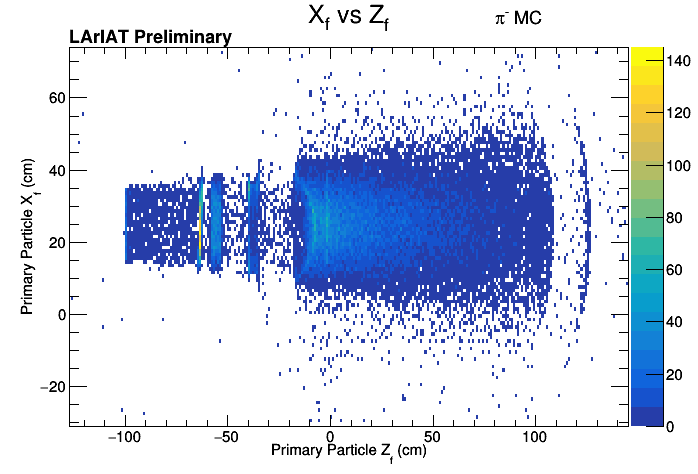
\includegraphics[scale=0.45]{./images/UnweightedXfvsZfupstreamzoom.png}
\caption{End point position for a sample of single particle $\pi^{-}$ MC showing the simulated upstream material and the interaction the pions can have with it.}
\label{fig:EndPointPionMCInBeamLine}
\end{figure}

This process obviously occurs in the data as well, and needs to be accounted for when taking the momentum of the particle measured from the wire chambers and extrapolating this to the TPC. In order to assess how much energy is loss for a pion traversing the material between Wire Chamber four and the front face of the active volume of the TPC, we take the $\pi$ MC and add up all the energy loss between the generation point ($z = -100$~cm) and the TPC ($z=0$~cm). Figure \ref{fig:EnergyLoss} shows the sum of all the energy loss for each pion prior to the particle entering the TPC. Any pion which does not have a trajectory which intercepts the TPC (e.g. interacts strongly in the upstream material) is excluded from this plot.

\begin{figure}[h!]
\centering
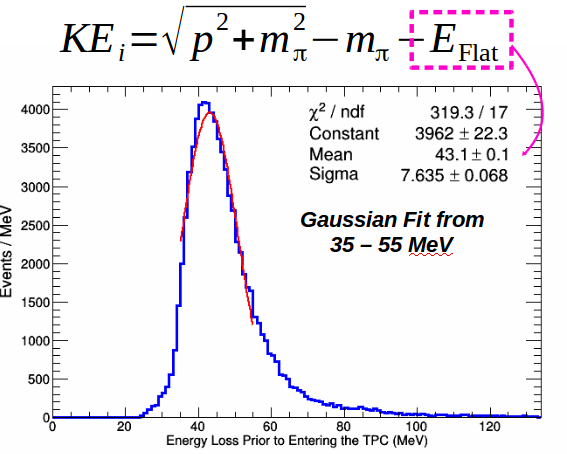
\includegraphics[scale=0.45]{./images/Eloss.png}
\caption{Energy loss from pions interacting in the simulated upstream material.}
\label{fig:EnergyLoss}
\end{figure}

Fitting the peak with a Gaussian, the most mean value is given as 40~MeV. The correction due to the energy loss from the upstream material is applied when calculating the initial kinetic energy as the term $E_{Flat}$